\documentclass[12pt]{article}
\usepackage[T1]{fontenc}
\usepackage{calc}
\usepackage{setspace}
\usepackage{multicol}
\usepackage{fancyheadings}

\usepackage{graphicx}
\usepackage{color}
\usepackage{rotating}
\usepackage{harvard}
\usepackage{aer}
\usepackage{aertt}
\usepackage{verbatim}

\setlength{\voffset}{0in}
\setlength{\topmargin}{0pt}
\setlength{\hoffset}{0pt}
\setlength{\oddsidemargin}{0pt}
\setlength{\headheight}{0pt}
\setlength{\headsep}{0.4in}
\setlength{\marginparsep}{0pt}
\setlength{\marginparwidth}{0pt}
\setlength{\marginparpush}{0pt}
\setlength{\footskip}{.1in}
\setlength{\textwidth}{6.5in}
\setlength{\textheight}{8.5in}
\setlength{\parskip}{0pc}

\renewcommand{\baselinestretch}{1.5}

\newcommand{\bi}{\begin{itemize}}
\newcommand{\ei}{\end{itemize}}
\newcommand{\be}{\begin{enumerate}}
\newcommand{\ee}{\end{enumerate}}
\newcommand{\bd}{\begin{description}}
\newcommand{\ed}{\end{description}}
\newcommand{\prbf}[1]{\textbf{#1}}
\newcommand{\prit}[1]{\textit{#1}}
\newcommand{\beq}{\begin{equation}}
\newcommand{\eeq}{\end{equation}}
\newcommand{\beqa}{\begin{eqnarray}}
\newcommand{\eeqa}{\end{eqnarray}}
\newcommand{\bdm}{\begin{displaymath}}
\newcommand{\edm}{\end{displaymath}}
\newcommand{\script}[1]{\begin{cal}#1\end{cal}}
\newcommand{\citee}[1]{\citename{#1} (\citeyear{#1})}
\newcommand{\h}[1]{\hat{#1}}
\newcommand{\ds}{\displaystyle}

\newcommand{\app}
{
\appendix
}

\newcommand{\appsection}[1]
{
\let\oldthesection\thesection
\renewcommand{\thesection}{Appendix \oldthesection}
\section{#1}\let\thesection\oldthesection
\renewcommand{\theequation}{\thesection\arabic{equation}}
\setcounter{equation}{0}
}

\pagestyle{plain}

\begin{document}

\begin{titlepage}
\begin{singlespace}
\title{Initial Expectations in New Keynesian Models with Learning\footnote{I am grateful for the advice and guidance of Eric Leeper, Kim Huynh, Brian Peterson, and Todd Walker; for useful conversations with Fabio Milani and Bruce Preston; and for comments by the participants of Indiana University economics department seminars.  All errors are my own.}}
\date{\today}
\author{
James Murray\footnote{\textit{Mailing address}: 1725 State St., La Crosse, WI  54601. \textit{Phone}: (608)785-5140.\newline  \textit{E-mail}: jmurray@uwlax.edu.}\\Department of Economics\\University of Wisconsin - La Crosse
}

\maketitle

\thispagestyle{empty}

\abstract{This paper examines how the estimation results for a standard New Keynesian model with constant gain least squares learning is sensitive to the stance taken on agents' beliefs at the beginning of the sample.  The New Keynesian model is estimated under rational expectations and under learning with three different frameworks for how expectations are set at the beginning of the sample.  The results show that initial beliefs can have an impact on the predictions of an estimated model; in fact previous literature has exposed this sensitivity to explain the changing volatility of output and inflation in the post-war United States.  The results indicate statistical evidence for adaptive learning, however the rational expectations framework performs at least as well as the learning frameworks, if not better, in in-sample and out-of-sample forecast error criteria.  Moreover, learning is not found to better explain time varying macroeconomic volatility any better than rational expectations.  Finally, impulse response functions from the estimated models show that the dynamics following a structural shock can depend crucially on how expectations are initialized and what information agents are assumed to have.
} \newline  

\noindent \textit{Keywords}: Learning, expectations, New Keynesian model, maximum likelihood. \\
\noindent \textit{JEL classification}: C13, E31, E50.
\end{singlespace}
\end{titlepage}
\newpage

\section{Introduction}
Recently there has been a growing amount of literature concerning the effects of least squares learning, a type of adaptive expectations mechanism, on empirical puzzles encountered in monetary economics.  Least squares learning is an expectations framework where agents in a model do not know the parameters that govern the economy and therefore form expectations by collecting past data and computing forecasts from least squares estimation results.  \citee{ow2005} show with a simple calibrated model and simulated impulse response functions that such a learning framework can cause prolonged periods of inflation, that would not occur under rational expectations, following an inflation shock.  Learning has also been suggested to be responsible for the slowdown in macroeconomic volatility since the middle 1980s, a phenomenon commonly referred to as the Great Moderation.  For example, \citee{ow2005b} suggest in another paper that the monetary authority forms their expectations by learning and was under-estimating the natural rate of unemployment during the 1970s, causing an incorrect prescription for expansionary monetary policy.  \citee{primiceri2006} takes this argument further and suggests that over the course of the 1970s and early 1980s the monetary authority gradually gained precision in their estimates, causing policy prescription to correctly adjust to stabilize output and inflation.

\citee{milani2007} has suggested that learning can better explain persistence in output and inflation in the context of a New Keynesian model better than traditional means of modeling persistence such as habit formation and inflation indexation.  \citename{milani2007} also estimates the size of the constant learning gain, the parameter responsible for the degree to which expectations evolve, and finds that expectations are adaptive over a post-war sample period.  

The results in \citee{milani2007} and \citee{primiceri2006} depend on calibrated values for expectations at the beginning of the sample.  Moreover, the dynamics predicted by learning can be influenced by the assumptions regarding agents information sets.  The purpose of this paper is to examine the role constant gain learning, a specific type of least squares learning, has on the predictions of an estimated standard New Keynesian model.  Moreover, this paper carefully considers different frameworks for how initial expectations are specified and what information agents are able to collect to form their forecasts.  Through examining forecast errors, rational expectations is shown to explain the data nearly as well, if not better, than the various learning frameworks.   Even so, the estimates for the learning gain indicate statistical evidence for adaptive expectations.  Impulse response functions are examined to determine the effects the various learning frameworks have on the dynamics of the model following a structural shock.  The results indicate that the impulse response functions can vary depending on the assumptions for agents' information sets and initial expectations.  Moreover, the findings indicate that learning can lead to some prolonged effects in output and inflation following a structural shock.

The results do not confirm, however, previous literature that suggests learning can explain periods of excessive volatility in inflation and output followed by the subsequent decline in volatility.  Evolution of the forecast errors over the sample indicate the rational expectations model and learning models all make similar errors, and all models make the largest errors during the 1970s and early 1980s when inflation and output were especially volatile.

The next section describes the basic setup of the New Keynesian model.  Section 3 describes the learning procedure and how learning is incorporated into a standard linear dynamic stochastic general equilibrium (DGSE) model.  Section 4 describes the estimation procedure and the issues involved in initializing expectations and determining agents' information sets.  Section 5 presents the results, and Section 6 concludes.

\section{Model}
Learning is examined within the context of a standard New Keynesian model.  The New Keynesian model is one of the most commonly used models in monetary economics as it provides a convenient framework to examine theoretical and empirical issues for monetary policy and inflation and output determination.  This section describes the set-up and log-linearization of the rational expectations model. In the next section the rational expectations are replaced by expectations under learning.\footnote{This is perhaps the most common way to incorporate learning into dynamic macroeconomic models.  However, as \citee{marcetsargent1989} point out and \citee{preston2005} further demonstrates, this method is not consistent with learning in the microfoundations of the model because the least squares expectations operator does not follow the law of iterated expectations, a property that is assumed when solving the model.}

The model consists of three sectors that describe consumer behavior, producer behavior under imperfectly flexible prices, and monetary policy.  The first sector is an equation or system of equations that describes optimal consumer behavior.  When this sector can be conveniently written in one equation, this is often called the ``IS equation''.  The second sector is a single equation, referred to as the Phillips curve, that describes optimal producer behavior when firms are subject to a pricing friction.  The final sector is the monetary authority, which is usually assumed to follow a simple nominal interest rate rule.  The sectors jointly determine the dynamics of the output gap (the percentage difference between real GDP and potential GDP), the inflation rate, and the nominal interest rate.  

\subsection{Consumers}
There are a continuum of consumer types and a continuum of intermediate good producers, each on the unit interval.  Each consumer type has a specific type of labor skill that can only be hired by a corresponding intermediate good firm.  It is assumed that there many consumers of each type so that no consumer has market power over their wage.  Moreover, it is assumed that there are the same number of consumers in each type, so that the output levels of intermediate goods do not depend on the distribution of consumer types.  Different intermediate goods firms may pay different wages, so labor income may be different for each consumer type.  To simplify the model, it is further assumed that there is a perfect asset market so despite differences in labor income, all consumers choose the same level of consumption.

Each consumer of type $i\in(0,1)$ chooses consumption, $c_t$, labor supply, $n_t(i)$, and purchases of real government bonds, $b_{t}(i)$, to maximize lifetime utility,
\beq \label{eq1:util} E_0 \sum_{t=0}^{\infty} \beta^t \left[ \frac{1}{1-\frac{1}{\sigma}} \xi_t \left(c_t - \eta c_{t-1}\right)^{1-\frac{1}{\sigma}} - \frac{1}{1+\frac{1}{\mu}} n_t(i)^{1+\frac{1}{\mu}} \right], \eeq
subject to the budget constraint, 
\beq \label{eq1:bc} c_t + b_t(i) = \frac{1+r_{t-1}}{1+\pi_t} b_{t-1}(i) + \frac{w_t(i)}{p_t} n_t(i) + \Pi_t - \tau_t. \eeq
where $\xi_t$ is an aggregate preference shock, $w_t(i)/p_t$ is the real wage paid to type $i$ labor; $\Pi_t$ is the total value of profits consumers earn by owning stock in firms, and $\tau_t$ is the real value of lump sum taxes.  The preference parameters are the intertemporal elasticity of substitution, denoted by $\sigma \in (0,\infty)$; the elasticity of labor supply, denoted by $\mu \in (0, \infty)$; and the degree of habit formation, denoted by $\eta \in [0,1)$.

When the degree of habit formation is greater than zero, consumers' utility from current consumption depends on their previous level of consumption.  Habit formation introduces persistence in consumption, and therefore output.  Significant output persistence is commonly found in empirical studies of DSGE models.  For example, \citee{smetswouters2005} find point estimates of habit formation close to unity.  Furthermore, \citee{fuhrer2000} finds that habit formation leads to ``hump-shaped'' impulse response functions, a characteristic commonly supported by U.S. and European data.  \citee{milani2007} finds a significant degree of habit formation, but only under rational expectations.  When estimating the model with constant gain learning, he finds an estimate for the degree of habit formation close to zero.   

Log-linearizing consumers' first order conditions leads to the following log-linear Euler equation,
\beq \label{eq1:lneuler} \h{\lambda}_{t} = E_t \h{\lambda}_{t+1} + \h{r}_t - E_t \pi_{t+1}, \eeq
where $\h{\lambda}_t$ is the percentage deviation from the steady state of the Lagrange multiplier on the budget constraint, (\ref{eq1:bc}), and is therefore interpreted as the marginal utility of real income.  A hat indicates the percentage deviation of a variable from its steady state.\footnote{A hat is omitted from $\pi_t$ because it is necessary to assume the steady state level of inflation is equal to zero when deriving the log-linear supply relationship.}  Utility maximization leads to the following log-linear marginal utility of income,
\beq \label{eq1:lnlambda} \h{\lambda}_t = \frac{1}{ (1-\beta \eta)(1-\eta)}\left[ \beta \eta \sigma E_t \h{c}_{t+1} - \sigma(1+\beta \eta^2) \h{c}_t + \sigma \eta \h{c}_{t-1} \right] + \left(\h{\xi}_t - \beta \eta E_t \h{\xi}_{t+1} \right). \eeq
The marginal utility of income, (\ref{eq1:lnlambda}), and the Euler equation, (\ref{eq1:lneuler}), make up the IS sector of the model.

\subsection{Producers}
There is one final good used for consumption which is sold in a perfectly competitive market and produced with a continuum of intermediate goods according to the production function,
\beq \label{eq1:yprod} y_t = \left[ \int_0^1 y_t(i)^{\frac{\theta-1}{\theta}} di \right]^{\frac{\theta}{\theta-1}}, \eeq
where $y_t$ is the output of the final good, $y_t(i)$ is the output of intermediate good $i$, and $\theta\in(1,\infty)$ is the elasticity of substitution in production.  Profit maximization leads to the following demand for each intermediate good,
\beq \label{eq1:yi} y_t(i) = \left[ \frac{p_t(i)}{p_t} \right]^{-\theta} y_t, \eeq
where $p_t(i)$ is the price of intermediate good $i$ and $p_t$ is the price of the final good.  Substituting equation (\ref{eq1:yi}) into equation (\ref{eq1:yprod}) leads to the following expression for the price of the final good in terms of the prices of intermediate goods,
\beq \label{eq1:pfinal} p_t = \left[ \int_0^1 p_t(i)^{1-\theta} di \right]^{\frac{1}{1-\theta}}. \eeq

Each intermediate good is sold in a monopolistically competitive market and is produced according to the production function, $y_t(i) = z_t n_t(i)$, where $z_t$ is an aggregate technology shock.  It can be shown that intermediate goods firms' optimal choices for labor demand and labor market clearing leads to the following aggregate log-linear marginal cost,
\beq \label{eq1:mc2} \h{\psi}_t = \frac{1}{\mu} \h{y}_t - \h{\lambda}_t - \left(\frac{1}{\mu} + 1\right) \h{z}_t. \eeq

Firm's pricing conditions are subject to the \citee{calvo1983} pricing friction, where only a constant fraction of firms are able to re-optimize their price in a given period.  The firms that are able to re-optimize their price is randomly determined, completely independently of firms' prices or any other characteristics or history.  I suppose that firms who are not able to re-optimize their price do adjust their price by a fraction, $\gamma \in [0,1)$, of the previous period's inflation rate.  A positive degree of price indexation introduces a source of persistence in inflation which is often found to be statistically significant when estimating New Keynesian models (see for example, \citename{smetswouters2005} (\citeyear{smetswouters2003}), (\citeyear{smetswouters2003}), (\citeyear{smetswouters2007}), and \citee{milani2007}).

Let $\omega \in (0,1)$ denote the fraction of firms that are not able to re-optimize their prices every period.  Since these firms are randomly determined, $\omega^T$ is the probability that a firm will not be able to re-optimize its price for $T$ consecutive periods.  A firm who is able to re-optimize chooses its price to maximize the following present discounted utility value of profits earned while the firm is unable to re-optimize its price again: 
\beq \label{eq1:intprofit}
E_t \sum_{T=0}^{\infty} \left(\omega \beta \right)^{T} \frac{\lambda_{t+T}}{\lambda_t}
\left\{ \left(\frac{p_{t}(i) \pi_{t+T}^{*}}{p_{t+T}}\right) y_{t+T}(i) - \Psi\left[y_{t+T}(i)\right] \right\},
\eeq
where $\Psi\left[y_{t+T}(i)\right]$ is the real total cost function of producing $y_{t+T}(i)$ units, given the optimal decision for labor, and $\pi_{t+T}^{*} = \prod_{j=1}^{T} (1+\gamma \pi_{t+j-1})$ is degree to which the firm's price is able to adjust according to inflation indexation.  It can be shown that the first order condition for $p_{t}(i)$ combined with the final good price index, equation (\ref{eq1:pfinal}), leads to the log-linear Phillips equation,\footnote{It is assumed during the log-linearization that there is a steady state for the price level, which implicitly assumes the steady state level of inflation is equal to zero.}
\beq \label{eq1:phillips} \pi_t = \frac{1}{1+\beta \gamma} \left[ \gamma \pi_{t-1} + \beta E_t \pi_{t+1} + \frac{\mu (1-\omega)(1-\omega \beta)}{\omega (\mu + \theta)} \h{\psi}_t \right]. \eeq

\subsection{Fully Flexible Prices}
The IS equations and Phillips equations can be re-written in terms of the difference from the outcome under fully flexible prices.  This allows the model to be taken to data on the output gap, the percentage deviation of real GDP from real potential GDP, as measured by the Congressional Budget office.  

Let $\tilde{y}_t = \h{y}_t - \h{y}_t^f$ and $\tilde{\lambda}_t = \h{\lambda}_t - \h{\lambda}_t^f$ denote the percentage deviation of output and marginal utility from their fully flexible price outcomes, where a superscript $f$ denotes the outcome under fully flexible prices.  Under flexible prices the linearized Euler equation, (\ref{eq1:lneuler}), and marginal utility of income, (\ref{eq1:lnlambda}), still hold.  Using these conditions and imposing goods market clearing that consumption is equal to output implies,
\beq \label{eq1:gapeuler} \tilde{\lambda}_{t} = E_t \tilde{\lambda}_{t+1} + \h{r}_t - E_t \pi_{t+1} - r_t^n, \eeq
\beq \label{eq1:gaplambda} \tilde{\lambda}_t = \frac{1}{ (1-\beta \eta)(1-\eta)}\left[ \beta \eta \sigma E_t \tilde{y}_{t+1} - \sigma(1+\beta \eta^2) \tilde{y}_t + \sigma \eta \tilde{y}_{t-1} \right], \eeq
where $r_t^n$ is the percentage deviation of the natural interest rate from its steady state.  The ``natural interest rate'' is the interest rate that would occur under fully flexible prices.  I suppose that $r_t^n$ follows the stochastic exogenous process,
\beq \label{eq1:natint} r_t^n = \rho_n r_{t-1}^n + \epsilon_{n,t}, \eeq
where $\epsilon_{n,t}$ is an independently and identically distributed shock.

When prices are fully flexible, it can be shown that intermediate goods firms will all choose the same price in a given period, and the marginal cost of production is constant, and therefore always will be equal to its steady state value.  Under fully flexible prices, equation (\ref{eq1:mc2}) implies,
\bdm \h{\psi}_t^f = \frac{1}{\mu} \h{y}_t^f - \h{\lambda}_t^f - \left(\frac{1}{\mu} + 1\right) \h{z}_t = 0. \edm
One can solve this equation for $\h{z}_t$ and substitute it back into the equation for marginal cost, (\ref{eq1:mc2}).  Plugging this expression for marginal cost into equation (\ref{eq1:phillips}) yields the following Phillips curve in terms of the output gap,
\bdm \label{eq1:phillips1} \pi_t = \frac{1}{1+\beta \gamma} \left[ \gamma \pi_{t-1} + \beta E_t \pi_{t+1} + \frac{(1-\omega)(1-\omega \beta)}{\omega (\mu + \theta)} (\tilde{y}_t - \mu \tilde{\lambda}_t) \right]. \edm
While this expression for the Phillips curve is not subject to a structural shock, when estimating the model by maximum likelihood it is convenient to have a shock here to avoid the problem of stochastic singularity.  The Phillips curve is amended with a ``cost-push'' shock so the form that is estimated is given by,
\beq \label{eq1:gapphillips} \pi_t = \frac{1}{1+\beta \gamma} \left[ \gamma \pi_{t-1} + \beta E_t \pi_{t+1} + \kappa (\tilde{y}_t - \mu \tilde{\lambda}_t) + u_t\right], \eeq
where $\kappa$ is the reduced form coefficient on the marginal cost and $u_t$ is an exogenous cost-push shock that evolves according to,
\beq \label{eq1:costpush} u_t = \rho_u u_{t-1} + \epsilon_{u,t}, \eeq
where $\epsilon_{u,t}$ is an independently and identically distributed shock.

\subsection{Monetary Policy}
The nominal interest rate is determined jointly with output and inflation by monetary policy.  In this paper I assume the monetary authority follows a \citee{taylor1993} type rule where the interest rate is set in response to expected output and inflation, with a preference for interest rate smoothing, according to,
\beq \label{eq1:taylor} \h{r}_t = \rho_r \h{r}_{t-1} + (1-\rho_r) \left(\psi_{\pi} E_t \pi_{t+1} + \psi_y E_t \tilde{y}_{t+1} \right) + \epsilon_{r,t} \eeq
where $\rho_r \in [0,1)$ is the degree of exogenous interest rate persistence, $\psi_{\pi} \in (0,\infty)$ is the degree to which monetary policy responds to expectations of future inflation above the steady state level of inflation, $\psi_y \in (0,\infty)$ is the degree to which monetary policy responds to the expected output gap, and $\epsilon_{r,t}$ is an independently and identically distributed exogenous monetary policy shock with mean zero and variance given by $\sigma_r^2$.  

Alternative policy rules may replace expected inflation and output with current or lagged realizations.  For example, \citee{mccallum1997} argues that a policy rule that depends on current realizations of output and inflation does not accurately depict actual information available to central banks when monetary policy decisions are made, since it takes about a full quarter to produce actual data on real GDP and price levels.  He argues that the monetary policy rule should instead be expressed as a function of past data.  The Taylor rule in (\ref{eq1:taylor}) is subject to this criticism under rational expectations, but it is shown in the next section that when agents learn, expectations of future variables are completely functions of past data.

\subsection{Complete Model}
The complete linear New Keynesian model is represented by ``IS relationship'', given in equations (\ref{eq1:gaplambda}) and (\ref{eq1:gapeuler}); the Phillips curve in equation (\ref{eq1:gapphillips}), and the Taylor rule in equation (\ref{eq1:taylor}).  These equations determine the dynamics of the output gap ($\tilde{y}_t$), the marginal utility of income gap ($\tilde{\lambda}_t$), the inflation rate ($\pi_t$), and the interest rate ($\h{r}_t$).  The model is subject to three structural shocks: the natural rate shock, which has an autoregressive evolution given in equation (\ref{eq1:natint}); the cost push shock, whose evolution is given in equation (\ref{eq1:costpush}), and the monetary policy shock.

\section{Learning}
The log-linearized model in the previous section can be expressed in the form,
\beq \label{eq1:sform} \Omega_{0} x_t = \Omega_{1} x_{t-1} + \Omega_{2} E_t^* x_{t+1} + \Psi v_t \eeq
\beq \label{eq1:sformv} v_t = A v_{t-1} + \epsilon_t, \eeq
where $x_t' = [\tilde{y}_t~ \tilde{\lambda}_t~ \pi_t~ \h{r}_t]'$, $v_t' = [r_t^n~ u_t~ \epsilon_{r,t}]'$, and $E_t^*$ denotes possibly non-rational expectations.  Under rational expectations, the solution of the model has the form,
\beq \label{eq1:solform} x_t = G x_{t-1} + H v_t, \eeq
where the elements of the matrices $G$ and $H$ are a function of the parameters of the model and may be determined by the method of undetermined coefficients.  Under rational expectations, agents know the parameters of the model and form the expectation,
\bdm E_t x_{t+1} = G x_t + H E_t v_{t+1}. \edm
Under learning, agents do not know the parameters of the model that make up the elements of matrices $G$ and $H$.  Instead, agents form expectations by estimating a linear model and using this model to make forecasts for $x_{t+1}$.  It is popular to assume that agents know the structure of the reduced form in equation (\ref{eq1:solform}), then collect data to and estimate $G$ and $H$ by least squares.  This method is employed in this paper, but there are five important questions to consider concerning agents information sets:
\be
\item What are the most recent observations agents have in their datasets?
\item Do agents collect data on structural shocks? 
\item If so, what are the most recent observations for structural shocks?
\item Do agents estimate a constant term?
\item Do agents include as explanatory variables those associated with a column of zeros in $G$?
\ee

I assume agents can only collect data for variables in $x_t$ up through the previous period.  This is both a realistic and greatly simplifying assumption.  While current information about interest rates are available in real life, data such as real GDP and price level released by statistical agencies such as the Bureau of Labor Statistics is typically available only months after the fact.  Assuming agents have only past data greatly simplifies solving the model since $x_t$ depends on agents' expectations.  Under learning, expectations are equal to least squares forecasts, which is a non-linear function of the data agents use.  Assuming $x_t$ is not part of this data avoids the problem of solving a complex, non-linear model.

This paper explores both answers to the second question on whether data on structural shocks are available to agents.  Since such data is not directly observable to an econometrician, it is quite realistic to suppose agents cannot observe this data either.  When agents only have data on $x_t$, they form estimates for the coefficient matrix $G$ and simply ignore the term with the structural shocks (this is appropriate since the unconditional expectation for $v_t$ is equal to zero).   

One of the goals of this paper is to identify the impact of learning on the predictions of an estimated New Keynesian model.  Under rational expectations agents know current period shocks, so to isolate the effects of learning from the effects of simply assuming a more limited information set I also examine the case when agents do have data on the current period structural shocks.  Since structural shocks are exogenous, there are no non-linearity issues in assuming agents have current period shocks.  Moreover, equation (\ref{eq1:solform}) shows that under rational expectations, assuming that agents can observe current period $x_t$ is equivalent to assuming agents have data up to the previous period for the state vector and data up to the current period for the structural shocks.  Therefore letting agents have access to data on current period shocks leads to the exact same information set under learning as rational expectations.

There is no constant term in the general form of the model, given in equation (\ref{eq1:sform}), or in the rational expectations solution of the model, equation (\ref{eq1:solform}), since all the variables in the New Keynesian model are expressed in percentage deviations from either the steady state or the flexible price outcome.  However, when agents learn, they are not endowed with the values of the parameters that govern the economy, so it is unreasonable to suppose agents know the steady state of the economy.  A constant term is augmented to agents regressions to capture this lack of knowledge.  Agents estimate the system,
\bdm x_t = g + G x_{t-1} + H v_t, \edm
or in the case when structural shocks are not observable,
\bdm x_t = g + G x_{t-1}. \edm

Finally, I assume that agents exclude from their datasets the variables in $x_t$ that correspond with a column of zeros in the rational expectations solution for $G$.  In terms of the New Keynesian model, the only variable that agents exclude is the marginal utility of income, $\tilde{\lambda}_t$.  The marginal utility of income does not include any predictive power that the output gap does not, so agents exclude this from their explanatory variables in their regression.  Agents do still forecast the marginal utility of income in order to make optimal consumption decisions according to the Euler equation, (\ref{eq1:gapeuler}).

Let $\Phi_t$ denote the time $t$ estimate of the all the coefficients to be estimated in the learning process.  These coefficients include a vector of constants, the non-zero columns in $G$, and all the columns in $H$ in the case where shocks are used as explanatory variables.  Let $Y_t$ denote the time $t$ dependent variables used in the learning process.  Since time $t$ data is not available to agents, $Y_t = x_{t-1}$.  Let $X_t$ denote the vector of time $t$ explanatory variables.  If agents include the stochastic shocks in their explanatory variables, $X_t' = [1~ x_{t-2}'~ v_{t-1}']$, otherwise $X_t' = [1~ x_{t-2}']$.  If agents use OLS they form the estimate,
\beq \label{eq1:Phi} \Phi_t' = \left( \frac{1}{t-1} \sum_{\tau=2}^{t} X_{\tau} X_{\tau}' \right)^{-1} \left( \frac{1}{t-1} \sum_{\tau=2}^{t} X_{\tau} Y_{\tau}' \right). \eeq 
The OLS estimate $\Phi_t$ can be rewritten into the convenient recursive form:
\beq \label{eq1:lnPhi} \Phi_t = \Phi_{t-1} + g_t (Y_{t} - \Phi_{t-1} X_{t}) X_{t}' R_t^{-1} ,\eeq
\beq \label{eq1:lnR} R_t = R_{t-1} + g_t (X_{t} X_{t}' - R_{t-1}), \eeq
where $g_t=1/(t-1)$ is the learning gain.\footnote{To show this, let $R_t = \frac{1}{t-1} \sum_{\tau=2}^{t} X_{\tau} X_{\tau}'$ and $\Phi' = R_t^{-1} \left( \frac{1}{t-1} \sum_{\tau=2}^{t} X_{\tau} Y_{\tau}' \right)$}  The recursive form demonstrates precisely how expectations are adaptive.  Agents take the previous period's estimates, $\Phi_{t-1}$ and $R_{t-1}$, and correct them according to the residual between the previous period's forecast and the new observation.  The amount of the correction depends on the learning gain.  The larger is the learning gain, the more expectations respond to the latest forecast error.  With OLS and infinite memory, the learning gain approaches zero as time approaches infinity, so the effect new observations have on updating the beliefs of $\Phi$ and $R$ diminish as the number of observations already in the sample approaches infinity.  

This paper instead examines the effects of constant gain learning, where the learning gain is assumed constant over time so that $g_t = g$.  This type of expectations formation is appealing because unlike OLS, it allows learning to explain macroeconomic dynamics in the long run.  This is a popular framework in the learning literature and is the same type of learning that \citee{ow2005} use to explain inflation scares, \citee{primiceri2006} uses to explain inflation volatility in the 1970s, and \citee{milani2007} uses to explain macroeconomic persistence.

Constant gain learning is equivalent to estimation by weighed least squares, where the most weight is given to the most recent observation and the weights decline geometrically with age.  This is a convenient framework to examine expectations when agents believe structural changes are possible.  Agents do not have any information as to what types of structural changes are possible, or with what probabilities.  Rather, they have constant suspicion that the way the economy operates may have changed, so most recent observations are given the most weight.  It has also been suggested, for example by \citee{evanshonka2001} and \citee{sargent1999}, that the constant gain learning algorithm in equations (\ref{eq1:lnPhi}) and (\ref{eq1:lnR}) closely resembles expectations when agents use ordinary least squares, but with a rolling window of data where the sample size is approximately $1/g$.  The constant gain learning algorithm is not identical to this scenario since it implies a weighted least squares procedure.  However, the weight an additional observation under the rolling window algorithm is equal to the inverse of the sample size, which is equal to the constant learning gain.  

Let $\h{g}_{0,t}$ denote the estimated constant term in $\Phi_t$, and let $\h{G}_t$ and $\h{H}_t$ denote the time $t$ estimate of $G$ and $H$, respectively, obtained from $\Phi_t$, where $\h{H}_t$ is simply set equal to zero in the case when structural shocks are not observable.  Agents' expectation of $x_{t+1}$ is given by, 
\beq \label{eq1:agfore} E_t^* x_{t+1} = \h{g}_{0,t} + \h{G}_t E_t^* x_t + \h{H} E_t v_{t+1} \eeq
Note that equation (\ref{eq1:agfore}) assumes that expectations about future shocks, $v_{t+1}$, are rational.  This is a common simplifying assumption made in learning models.  It is possible to allow agents to also estimate the coefficients in the shock process, but the dynamics deriving from this additional complication are negligible.  Since time $t$ observations are not yet available to agents, agents must also estimate $x_t$ by least squares.  The time $t$ estimate of $x_t$ is given by,
\beq \label{eq1:agfore1} E_t x_t^* = \h{g}_{0,t} + \h{G}_t x_{t-1} + \h{H} v_t. \eeq
Plugging this into equation (\ref{eq1:agfore}) yields,
\beq \label{eq1:agfore2} E_t^* x_{t+1} = (I + \h{G}_t)\h{g}_{0,t} + \h{G}_t^2 x_{t-1} + \left(\h{G}_t \h{H}_t + \h{H}_t A \right) v_t. \eeq

Plugging the agents' forecast, (\ref{eq1:agfore2}), into the structural form of the model, (\ref{eq1:sform}), leads to the following actual law of motion for $x_t$,
\beq \label{eq1:alm} x_t = \Omega_0^{-1}\Omega_{2}\left(I+\h{G}_t\right)\h{g}_{0,t} + \Omega_0^{-1} \left(\Omega_{1} + \Omega_{2} \h{G}_t^2 \right) x_{t-1}  + \Omega_0^{-1} \left[ \Psi + \Omega_2 \left(\h{G}_t \h{H}_t + \h{H}_t A \right) \right] v_t. \eeq

\section{Estimation}
\subsection{Maximum Likelihood}
The model is estimated with quarterly U.S. data from 1960:Q1 through 2007:Q1 on the output gap, as measured by the Congressional Budget Office, the inflation rate of the consumer price index, and the federal funds rate.  The model is estimated by maximum likelihood using the Kalman filter procedure described by \citee{hamilton} that maps the state equations (\ref{eq1:alm}) and (\ref{eq1:sformv}) and a system of observation equations to a log-likelihood function.  The observation equations are given by,
\bdm \begin{array}{c} \label{eq1:obs}  
\ds GAP_t = 100 \tilde{y}_t, \\
\ds INF_t = \pi^{*} + 400\pi_t, \\
\ds FF_t = r^{*} + \pi^* + 400\h{r}_t,
\end{array}
\edm
where $GAP_t$ denotes data on the output gap, $INF_t$ denotes data on the annualized quarterly inflation rate, and $FF_t$ denotes the annualized quarterly federal funds rate.  The state variables are multiplied by $100$ to convert the decimals into percentages, and the inflation rate and federal funds rate are further multiplied by $4$ to convert the quarterly rates to annualized rates.  The New Keynesian model assumes that the steady state inflation rate is equal to zero, but since this is not likely the case in the data, the annualized steady state inflation rate, given by  $\pi^*$, is estimated along with the other parameters of the model.  The steady state gross real interest rate is set equal to the inverse of the discount factor; therefore $r^* = 400(1/\beta-1)$.

The log-likelihood is maximized with respect to the learning gain, $g$; the New Keynesian parameters $\eta$, $\sigma^{-1}$, $\gamma$, $\rho_r$, $\psi_y$, $\psi_{\pi}$, $\rho_n$, $\rho_u$, $\sigma_n$, $\sigma_u$, and $\sigma_r$; and the steady state inflation rate, $\pi^*$.  Instead of estimating the intertemporal elasticity of substitution, preliminary results indicated very elastic intertemporal substitution effects so it is easier to identify the inverse of this parameter.  Three parameters are not estimated.  The discount factor, $\beta$, is set equal to $0.9925$.  This corresponds to a steady state annual real interest rate of 3\% which is close to the average difference between the federal funds rate and the inflation rate over the sample period.  Preliminary results indicated difficulty in identifying the elasticity of labor supply, $\mu$.  The only place this parameter appears in the model is on the Phillips curve multiplying the marginal utility of income, $\tilde{\lambda}_t$.  Equation (\ref{eq1:gaplambda}) shows that when carrying out this multiplication, $\mu$ and $\sigma$ appear multiplicatively, causing weak identification.  Therefore, the elasticity of labor supply is set equal to zero.  This implies that there are no changes in labor supply decisions that effect firms' marginal costs, and therefore there are no changes in labor supply that arise from firms altering pricing decisions.  Finally, the coefficient on the output gap in the Phillips curve, $\kappa$, is set equal to 0.1.  Preliminary results indicated estimates of $\kappa$ infinitely close to zero with a very high degree of precision, which has the unrealistic implication that prices are completely fixed for all time.  \citee{ireland_tech_2004} reports the same difficulty and also sets $\kappa=0.1$ prior to estimating the model.

\subsection{Initial Conditions}
Before estimating the model, it is necessary to specify initial conditions for the learning process given in equations (\ref{eq1:lnPhi}) and (\ref{eq1:lnR}).  Unlike specifying initial conditions for the Kalman filtering procedure, the choices for initial learning matrices, $\Phi_0$ and $R_{0}$, can have a dramatic effect on the estimation results.  Despite this dependence, there is little general consensus for how initial expectations should be specified.

\citee{williams2003} shows that using the rational expectations solution for initial expectations produces nearly identical dynamics as assuming expectations are rational throughout the sample.  Given the model is E-stable, this result is not too surprising.  If the conditions for E-stability are met, under a decreasing learning gain consistent with OLS, the model will converge to the rational expectations solution when in the neighborhood of this solution.  \citename{williams2003} shows with simulations that with a constant gain, the dynamics under learning do not significantly differ than under rational expectations.

Most initialization methods are therefore based on pre-sample evidence.  \citee{slobodyan_wouters2007} estimate the rational expectations version of the model on pre-sample data, and use the implied expectations as the initial condition for the sample.  \citee{milani2007} sets initial expectations based on statistical evidence with de-meaned pre-sample data, with a few exceptions.  For example he argues that agents perceived zero persistence in inflation at the beginning of the sample, when pre-sample evidence indicated it was low.  Moreover, he assumes agents do observe structural shocks and so sets the initial coefficients in $H$ equal to zero.  \citee{primiceri2006} calibrates initial conditions with the argument that the initial conditions are close to observed pre-sample evidence, and that the initial conditions describe well the behavior of the economy in the opening periods of the sample.  

In this paper, I examine the following four specifications for how agents form expectations, and how expectations are initialized:
\bd
\item Case 1.  Rational expectations.  
\item Case 2.  Learning with observable shocks and initial conditions set equal to rational expectations.
\item Case 3.  Learning without observable shocks and initial conditions set equal to rational expectations.
\item Case 4.  Learning without observable shocks and initial conditions set equal to pre-sample evidence.
\ed

Rational expectations is estimated as a baseline case for which to make comparisons.  Case 2 can be viewed as the smallest step away from rational expectations.  Agents have the same information set and expectations at the beginning of the sample.  This implies that rational expectations is actually the special case of this learning framework where the learning gain is equal to zero.  As the learning gain is estimated jointly with the other parameters of the model, the statistical significance of this parameter from zero can formally reject or fail to reject the null hypothesis that expectations are rational.

Case 3 makes another incremental step away from rational expectations.  Agents again learn according to constant gain least squares, and their initial conditions for the learning matrices are equal to the rational expectations values, but agents are not able to collect data on past shocks in order to use them as explanatory variables.  Due to this difference, Case 3 does not nest rational expectations.

Case 4 assumes the agents have the same information set as Case 3, but the initial conditions for the learning process matrices are different from the rational expectations solution.  The initial conditions are set equal to constant gain least squares estimates from pre-sample data.  Equations (\ref{eq1:lnPhi}) and (\ref{eq1:lnR}) describe the least squares learning process with any given learning gain, $g_t$.  When the learning gain is constant, repeated substitution of these equations can show that the learning matrices are given by,
\beq \label{eq1:Rsum} R_t = \sum_{\tau=0}^{t-1} \left(1-g\right)^t X_{t-\tau} X_{t-\tau}' \eeq
\beq \label{eq1:Phisum} \Phi_t = \left( \sum_{\tau=0}^{t-1} \left(1-g\right)^t X_{t-\tau} X_{t-\tau}' \right)^{-1} \left( \sum_{\tau=0}^{t-1} \left(1-g\right)^t X_{t-\tau} Y_{t-\tau}' \right) \eeq

Pre-sample data on the output gap, inflation rate, and federal funds rate are collected for the period 1954:Q3 through 1959:Q4.  Pre-sample data on the output gap is divided by 100 to convert it to pre-sample data for $\tilde{y}_t$.  The steady state levels for the inflation rate and nominal interest rate are removed from pre-sample data on the inflation rate and federal funds rate and these are divided by 400 to be put in terms of quarterly rates in the model.  The weighted least squares procedure in equations (\ref{eq1:Rsum}) and (\ref{eq1:Phisum}) is run on this pre-sample data to form matrices for $\Phi_0$ and $R_0$ for the beginning sample period 1960:Q1. 

\section{Results}

In this section I present the maximum likelihood estimation results for each of the four expectations frameworks.  To determine the role learning, initial expectations, and agents information sets have on the estimation results I look at the parameter results for each model in turn.  After understanding differences in parameter estimates I compare the relative fit of the models in terms of in-sample residuals and out-of-sample forecast errors.  Finally I show the roles the structural shocks play on the dynamics of model by examining impulse response functions and the predicted paths of the structural shocks over the sample period.

\subsection{Parameter Estimates}

\noindent \textbf{Case 1:  Rational Expectations}

Table \ref{tb:parms} shows the parameter estimates for all four specifications.  The first two columns are the results for the rational expectations model.  The results show habit formation is a very strong source of output persistence, with $\eta=0.99$.  The high estimate for habit formation is similar to \citename{smetswouters2005} (\citeyear{smetswouters2005}) and (\citeyear{smetswouters2007}) estimates from a larger New Keynesian estimated by Bayesian methods on U.S. data.  This result is also consistent with \citee{milani2007} finding that habit formation is significant when expectations are rational.  Despite the evidence for strong persistence in output, the estimated degree of price indexation is essentially equal to zero.  This is in contrast with \citename{smetswouters2005} and \citename{milani2007} who find degrees of price indexation very close to unity.  However, estimates for these degrees of persistence vary substantially across the empirical macroeconomics literature.  For example, \citee{ireland_tech_2004} estimates a similar model by maximum likelihood and finds small degrees of persistence in both output and inflation.  \citee{nasonsmith2005} use method of moments procedures to identify the Phillips curve and find point estimates for indexation close to 0.3.  \citee{csb2005} also use method of moments procedures and indexation is equal to 0.0.

The inverse intertemporal elasticity of substitution is $\sigma^{-1}=0.0015$ which is very small compared to much of the macroeconomics literature.  This implies that consumption decisions are very sensitive to changes in the expected real interest rate.  \citee{milani2007} for example finds an estimate for the inverse elasticity of substitution approximately equal to $0.26$ when expectations are rational.  Other papers find much higher estimates.  \citee{giannoni_woodford_2003} find the inverse elasticity approximately equal to $1.51$, and \citee{smetswouters2005} find this parameter approximately equal to $1.62$.  Some empirical work, such as \citee{ireland_tech_2004}, simply uses a log utility function which implicitly assumes the elasticity is equal to 1.  It will be seen in the cases below that the estimate for this parameter is sensitive to the expectations framework.\\

\noindent \textbf{Case 2:  Learning with RE Initial Conditions}

The next two columns of Table \ref{tb:parms} show the parameter estimates under learning, when agents have the same information set as rational expectations and when initial expectations are set equal to the rational expectations solution.  As mentioned above, rational expectations is the special case of this model where the constant learning gain is equal to zero.  The estimate for the learning gain is small, $g=0.0119$, but is statistically significantly greater than zero, which implies significant statistical evidence for learning.  This learning gain corresponds to agents using approximately the last 84 observations to form their expectations, or about 21 years of data.  

Many parameters estimates are very different than under rational expectations.  The degree of habit formation dropped to about $\eta=0.65$ and the degree of inflation indexation increased dramatically from zero to $\gamma=0.71$.  This implies when agents learn, past inflation is significant in explaining forecasts for future inflation.  The inverse elasticity of substitution jumped to $\sigma^{-1} = 0.42$, which is closer to other estimates found in the literature.  The lower intertemporal elasticity of substitution implies that consumption decisions are less responsive to the expected real interest rate.  The monetary policy parameters also indicate that dynamics in the data are less responsive to expectations under learning.  The response of monetary policy to expected output and expected inflation decreased to $\psi_y=0.08$ and $\psi_{\pi}=1.74$, respectively. \\

\noindent \textbf{Case 3:  Learning with Unobservable Shocks and RE Initial Conditions}

In the next learning case agents do not collect data on structural shocks.  Because shocks cannot directly influence expectations, all other things remaining the same, agents' forecasts should be less volatile.  The fourth and fifth columns of results in Table \ref{tb:parms} show the parameter estimates for this framework.  The learning gain is approximately, $g=0.0202$, which is nearly twice the size as in Case 2, and given the small standard errors, the estimate is significantly higher.  Since the shocks do not directly influence the volatility of expectations, the estimation results predict volatility in expectations is due to a higher learning gain.  This difference in the learning gain may appear small, but when interpreting it from the viewpoint of the number of past observations agents use helps put it in perspective; in Case 3 agents use about 50 observations to form their expectations, or just over 12 years of data.

The parameter estimates for inverse intertemporal elasticity of substitution and monetary policy parameters indicate that expectations play a larger role in inflation and output determination when agents do not observe structural shocks.  The inverse elasticity of substitution is $\sigma^{-1}=0.03$ which is smaller than in Case 2, but not nearly as small as under rational expectations.  Monetary policy parameters indicate stronger responses to expectations of inflation and the output gap, but still predict responses smaller than rational expectations.  

Assuming learning with a limited information set therefore still leads to the conclusion that inflation and output dynamics are less responsive under learning than under rational expectations.  However, the limited information set leads to greater volatility of expectations and greater sensitivity of consumption choices and monetary policy to expectations than under learning with a full information set.

\noindent \textbf{Case 4:  Learning with Pre-Sample Initial Conditions} 

The final case uses the same limited information set as Case 3, but sets expectations for the beginning sample period equal to pre-sample weighted least squares results.  The estimate for the learning gain is approximately $g=0.0175$ which corresponds to a rolling window of over 57 observations or just over 14 years of data.  Again the learning gain is statistically significantly greater than zero.  This implies that expectations are adaptive over the sample period.  

The estimates for the degrees of persistence are all significantly positive, but are not so close to unity.  Habit formation is $\eta=0.71$ and inflation indexation is $\gamma=0.63$.  This is in direct contrast to the \citee{milani2007} finding that these degrees of persistence are significant under rational expectations, but learning causes these to fall close to zero.  One possible explanation for the difference in these findings is the estimation procedure.  That paper uses Bayesian methods, whereas this paper uses maximum likelihood.  The initial conditions for expectations are also somewhat different.  \citename{milani2007} calibrates the initial expectations according to pre-sample estimation results from a first order vector autoregression (VAR(1)), but with some exceptions.  In his paper, initial expectations for inflation persistence are set equal to zero, output gap persistence is set below pre-sample evidence, and the sensitivity of inflation to the output gap is set above pre-sample sample evidence.  Moreover, the initial conditions based on pre-sample evidence for Case 4 of this paper is not set according to pre-sample VAR(1), but the pre-sample results from the weighted least squares vector autoregression given in equation (\ref{eq1:Phisum}) that is consistent with constant gain learning, for a given estimate of the learning gain.

\subsection{Model Fit Comparisons}

Given the different predictions of the four models, I turn to examine how well each model fits the data, and examine whether any of the learning models provides a better fit to the data during periods of the sample that is characterized by excess volatility, as it has been proposed by some authors that learning may help explain run-ups of inflation and subsequent declines.  The first three rows of Table \ref{tb:rmse} show the root mean squared residuals for each model.  The results indicate a very similar performance of all four models for all three variables.  The best performing model is actually the rational expectations model, but the improvement is very small.  

To determine whether the learning models can explain the time varying volatility in macroeconomic activity throughout the sample, the bottom three rows of Table \ref{tb:rmse} report the autocorrelation of the square of the residuals.  If a model is well specified and can explain changes in volatility in the data, then the volatility of the residuals should be constant throughout the sample and therefore the autocorrelation should equal zero.  The autocorrelation of the squared residuals are small but do indicate some persistence in volatility of the residuals.  The best performing model under this criteria for the output gap and federal funds rate is the learning model based on pre-sample initial conditions.  The autocorrelation for the output gap in Case 4 is approximately $0.09$, compared to values above $0.13$ in the other frameworks.  There is a small improvement in the autocorrelation for the federal funds rate, but it is still significantly above zero.  The best performing model for inflation using this criteria is Case 3, learning when agents do not have data on the structural shocks.  In this case the autocorrelation of the residuals is approximately $0.11$ compared to values of about $0.18$ and above for the other cases.

To see where the models are making their largest errors, Figure \ref{fg:fe} shows the plots of the forecast errors over the sample period for each of models.  The shaded regions indicate periods of recession as determined by the National Bureau of Economic Research.  The numbers in parentheses for the learning models are the correlation with the evolution of the forecast errors predicted by the rational expectations model.  Looking across the figure one can see the forecast errors for all the variables for all the learning frameworks are highly correlated with the forecast errors under rational expectations.  This implies that none of the learning models can explain any better the changes in macroeconomic volatility than the rational expectations model.  The largest forecast errors for the output gap are made in the recessions of the 1970s and early 1980s, the period characterized by high inflation and relatively large macroeconomic volatility.  The forecast errors for the output gap become relatively small after 1984 for every model, the period commonly referred to in the empirical monetary literature as the Great Moderation.  The forecast errors for inflation similarly are largest in the middle 1970s and the early 1980s, then become relatively smaller.

The models all have similar in-sample performance, but to to determine if learning dynamics can better explain data out-of-sample, the models are re-estimated using data from 1960:Q1 through 1989:Q4 and using these sets of parameters, the models are forecast over 1990:Q1 through 2008:Q1 for long horizons.  Figure \ref{fg:rmse} shows the root mean squared error of the out-of-sample forecast errors for forecast horizons of one quarter through 12 quarters.  The best performing model for the output gap for forecast horizons 1 quarter through 6 quarters is the rational expectations model.  However, at longer horizons, the learning model with expectations based on pre-sample data, is the best performing model.  The same is not true for inflation and interest rate forecasts.  For these variables, Case 4 is by far the worst performing model over the entire three year forecast horizon.  For all three variables rational expectations and learning under Cases 2 and 3 have very similar out-of-sample performance over the forecast horizon.

\subsection{Structural Shocks}

Despite the mixed performance of the four models in in-sample and out-of-sample fit, the significance of the learning gain combined with the differences in the parameter estimates could lead to different predictions for the relative importance of the structural shocks in explaining the data.  Figure \ref{fg:shocks} shows the estimated evolutions for the structural shocks, which are computed using the Kalman smoothing algorithm proposed by \citee{jong1989}.  Again, periods of recession in the United States are shaded and the correlation of the shocks in the learning models with the rational expectations model are shown in parentheses.  The correlations indicate there are some similarities in the predictions of the models, but the correlations are not quite so high as they are for the forecast errors.  

The natural rate shock is highly correlated over the four models.  The largest volatility of the natural rate shock is during the 1970s and early 1980s.  The natural rate shock also appears responsible for the recession in 2001.  The scale of the natural rate shocks show that Case 3 predicts the largest volatility this shock.  This is the case when expectations are least volatile because expectations are initialized to the rational expectations solution, and structural shocks do not directly impact expectations.  The cost push shock is somewhat correlated across the four models.  The shock is more persistent under rational expectations, but all the models predict the largest shocks come during the periods of stagflation in the middle 1970s and early 1980s.  The monetary policy shock shows that all models completely fail to deliver the change in monetary policy that occurred after Paul Volcker became chairman of the Federal Reserve.  Recall, previous authors such as \citee{primiceri2006} and \citee{ow2005b} have suggested that the change in monetary policy was due to changes in expectations caused by learning.  The results in this paper do not support such a claim.  Instead the models predict very volatile monetary policy shocks starting in late 1979 and become very small after 1984.

Figures \ref{fg:irf_nat}, \ref{fg:irf_cost}, and \ref{fg:irf_mp} show the predicted impulse response functions that arise from a one standard deviation shock to each of the structural shocks.  Impulse responses for learning models depend on the values of the learning matrices $\Phi_t$ and $R_t$ at the time of the impulse.  The impulse response functions computed in this paper are for the state of the learning matrices at the first quarter of 2008, the last period of the sample.  If the learning matrices are not equal to the rational expectations solution, then even in the absence of shocks the state variables evolve as expectations converge to the rational expectations solution.  Therefore, to expose only the impact of the shocks, the plots in Figures \ref{fg:irf_nat}, \ref{fg:irf_cost}, and \ref{fg:irf_mp} show the difference between the evolution of the variables after the shock and the evolution the variables would take in the absence of any shocks.

Figure \ref{fg:irf_nat} shows the impulse responds functions for the natural rate shock.  The unit these are measured in is the percentage deviation of each variable from its steady state.  The results show that learning can create significant ``hump-shaped'' impulse responses, especially in Cases 3 and 4 when agents do not have data on structural shocks.  The results indicate that Cases 3 and 4 create the largest and most prolonged effects following a shock.  Because in these cases agents do not have data on structural shocks, expectations are only influenced indirectly through the effect the shocks have on the state variables.  As time progresses the realizations of these state variables become data in agents regressions, and therefore shocks can influence expectations for long periods of time.  In Case 2, agents can see the structural shock and they know it is temporary, therefore a shock does not influence expectations over a long horizon.

Figure \ref{fg:irf_cost} shows the impulse responses due to a cost push shock.  The response to inflation is very similar over all three models, with the exception of Case 4 in which inflation dies down significantly after about 6 periods, but takes a very long time to completely converge to the steady state.  This finding is in contrast with \citee{ow2005} who suggest using simulated impulse response functions from a calibrated model that an inflation shock can lead to prolonged periods of inflation.  The bottom row of graphs in Figure \ref{fg:irf_cost} shows that initial expectations can lead to a very different prediction for the impact of the cost-push shock.  Instead of output decreasing due to higher costs, expectations by the end of the sample are at such a point that the shock causes output to increase for a prolonged period of time, which leads to a very different path for the interest rate.  This would be consistent if the increase in inflation caused by the cost push shock is instead interpreted by agents as an increase in demand.

Finally, Figure \ref{fg:irf_mp} shows the impulse responses from a contractionary monetary policy shock.  The shape of the impulse responses in Cases 1 and 2 are very similar.  However, the scale indicates that the negative impact on the output gap is much larger in Case 2 than under rational expectations.  The response to the output gap in Cases 3 and 4 is much longer lived, and appears to have a oscillatory pattern after many years.  Again Case 4 expectations at the end of the sample are in such a state that leads to a very different response to inflation.  The contractionary monetary shock causes only a small one period decrease in the inflation rate, as the increase in interest rate causes an intertemporal substitution effect that decreases demand.  The subsequent positive effect on inflation and continued negative effect on output is consistent with agents perceiving the change in interest rate as a response to a negative shock to supply.  

\section{Conclusion}

Constant gain learning is not found to out-perform rational expectations in the context of an estimated standard Keynesian model.  Previous research has suggested that constant gain learning can explain periods of prolonged inflation, run-ups of inflation and volatility and subsequent decline, and macroeconomic persistence.  These claims are tested in the context of the New Keynesian model, the most popular specification for monetary models for the use of estimating and examining the impacts of monetary policy on the economy.  To examine the effects of learning, initial expectations, and information sets, the rational expectations model is estimated along with three specifications for learning that differ on the assumed expectations at the beginning of the sample and whether agents can observe structural shocks.

Estimation results show that the learning gain is statistically significant in every case, indicating statistical evidence that expectations are not rational and are indeed adaptive.  Moreover, the different models deliver very different parameter estimates that are responsible for the impact expectations have on consumption behavior and monetary policy.  However, when comparing the models on criteria for in-sample and out-of-sample forecast errors, the rational expectations model delivered nearly as good as performance of the learning models, and compared to a learning model with initial expectations set to pre-sample evidence, the rational expectations model greatly out-perform the learning model in out-of-sample fit.

Analysis of impulse response functions showed despite the weak evidence for differences in fit, learning can have very different predictions for the effects structural shocks have on the dynamics of the model.  When agents are assumed to not be able to collect data on structural shocks, the shocks produce prolonged impulse responses.  Moreover, even the directions of some of the impulse response functions were shown to be quite sensitive to initial expectations.

\newpage
\nocite{*}
\bibliographystyle{econometrica}
\bibliography{initexp.bib}
\newpage
\begin{sidewaystable}
\begin{small}
\begin{center}
\caption{Maximum Likelihood Parameter Estimates${}^{*}$}\label{tb:parms}
\vspace*{1pc}
\begin{tabular}{l|c|r@{.}lr@{.}l|r@{.}lr@{.}l|r@{.}lr@{.}l|r@{.}lr@{.}l} \hline
Description & Parameter & \multicolumn{4}{|c|}{Case 1} & \multicolumn{4}{|c|}{Case 2} & \multicolumn{4}{|c|}{Case 3} & \multicolumn{4}{|c}{Case 4} \\ \hline 
Habit Persistence & $\eta$ & 0&7737 & (0&0651) & 0&7933 & (0&0660) & 0&9992 & (0&0001) & 0&7381 & (0&1897) \\  
Inverse IES & $\sigma^{-1}$ & 0&2098 & (0&1303) & 0&1952 & (0&1147) & 0&0000 & (0&0000) & 0&1113 & (0&1722) \\  
Phillips Slope & $\kappa$ & 0&0500 & (0&0000) & 0&0500 & (0&0000) & 0&0500 & (0&0000) & 0&0500 & (0&0000) \\  
Price Indexation & $\gamma$ & 0&7997 & (0&0406) & 0&7665 & (0&0604) & 0&6943 & (0&0462) & 1&0000 & (0&0000) \\  
MP Persistence & $\rho_r$ & 0&8491 & (0&0191) & 0&7952 & (0&0114) & 0&8997 & (0&0388) & 0&8623 & (0&0341) \\  
MP Output Gap & $\psi_y$ & 0&3033 & (0&0825) & 0&0976 & (0&0279) & 0&9484 & (0&4238) & 0&3165 & (0&1065) \\  
MP Inflation & $\psi_\pi$ & 2&8011 & (0&3829) & 1&6838 & (0&0885) & 3&0826 & (0&9868) & 1&2242 & (0&1446)  \\  
Natural Rate Pers. & $\rho_{n}$ & 0&8093 & (0&0294) & 0&8206 & (0&0063) & 0&6333 & (0&0279) & 0&3341 & (0&0415) \\  
Cost Push Pers. & $\rho_{u}$ & 0&0000 & (0&0442) & 0&0000 & (0&0017) & 0&0000 & (0&0464) & 0&0000 & (0&0379) \\  
Natural Rate Std. Dev. & $\sigma_{n}$ & 0&0064 & (0&0009) & 0&0047 & (0&0000) & 0&0180 & (0&0025) & 0&0188 & (0&0029)  \\  
Cost Push Std. Dev. & $\sigma_{u}$ & 0&0066 & (0&0002) & 0&0067 & (0&0003) & 0&0097 & (0&0003) & 0&0115 & (0&0002) \\  
Policy Shock Std. Dev. & $\sigma_{r}$ & 0&0031 & (0&0000) & 0&0027 & (0&0000) & 0&0030 & (0&0000) & 0&0029 & (0&0000)  \\  
Steady State Inlfation & $\pi^{*}$ & 3&8599 & (0&0000) & 3&8599 & (0&0000) & 3&8599 & (0&0000) & 3&8599 & (0&0000) \\  
Learning Gain & $g$ & \multicolumn{2}{|c}{--} & \multicolumn{2}{c|}{--} & 0&0209 & (0&0021) & 0&0152 & (0&0013) & 0&0000 & (0&0000)  \\ \hline 
\multicolumn{18}{p{7.5in}}{${}^{*}$ Maximum likelihood estimates for sample period 1960:Q1 through 2008:Q1.  Values in parentheses are the standard errors of the estimates.}
\end{tabular}
\end{center}
\end{small}
\end{sidewaystable}

\begin{table}
\caption{Model Fit Comparisons}\label{tb:rmse}
\begin{center}
\begin{tabular}{|l|cccc|}\hline
 & \multicolumn{4}{|c|}{Root Mean Squared Error} \\ 
 & Case 1 & Case 2 & Case 3 & Case 4 \\ \hline
Output Gap & 0.7757 & 0.7905 & 0.8012 & 0.7792 \\ 
Inflation & 2.3474 & 2.2863 & 2.2978 & 2.3092 \\ 
Federal Funds Rate & 1.2327 & 1.2392 & 1.2283 & 1.2118 \\ \hline 
 & \multicolumn{4}{|c|}{Autocorrelation Squared Error} \\ 
 & Case 1 & Case 2 & Case 3 & Case 4 \\ \hline
Output Gap & 0.1610 & 0.2080 & 0.1329 & 0.0387 \\ 
Inflation & 0.2058 & 0.1562 & 0.2125 & 0.2526 \\ 
Federal Funds Rate & 0.3665 & 0.1856 & 0.4164 & 0.4092 \\ \hline 
\end{tabular}
\end{center}
\end{table}

\begin{figure}
\caption{Forecast Errors}\label{fg:fe}\vspace*{1pc}
\begin{tabular}{ccc}
\multicolumn{3}{c}{Case 1: Rational Expectations} \\ 
Output Gap & Inflation & Fed Funds \\
\includegraphics[scale=0.28]{results_re/output_err.png} & 
\includegraphics[scale=0.28]{results_re/inflation_err.png} & 
\includegraphics[scale=0.28]{results_re/fedfunds_err.png} \\ \\ 
 
\multicolumn{3}{c}{Case 2: Learing with RE Initial Conditions} \\ 
Output Gap (0.9724) & Inflation (0.9492) & Fed Funds (0.9525) \\
\includegraphics[scale=0.28]{results_reallinit/output_err.png} & 
\includegraphics[scale=0.28]{results_reallinit/inflation_err.png} & 
\includegraphics[scale=0.28]{results_reallinit/fedfunds_err.png} \\ \\ 
 
\multicolumn{3}{c}{Case 3: Learing with RE Initial Conditions, Shocks Unobservable} \\ 
Output Gap (0.9329) & Inflation (0.9474) & Fed Funds (0.9461) \\
\includegraphics[scale=0.28]{results_reinit/output_err.png} & 
\includegraphics[scale=0.28]{results_reinit/inflation_err.png} & 
\includegraphics[scale=0.28]{results_reinit/fedfunds_err.png} \\ \\ 
 
\multicolumn{3}{c}{Case 4: Learning with Unobservable Shocks and Pre-Sample Initial Conditions} \\ 
Output Gap (0.9219) & Inflation (0.9121) & Fed Funds (0.9586) \\
\includegraphics[scale=0.28]{results_wlsinit/output_err.png} & 
\includegraphics[scale=0.28]{results_wlsinit/inflation_err.png} & 
\includegraphics[scale=0.28]{results_wlsinit/fedfunds_err.png} \\ \\ 
 
\end{tabular}
\end{figure}

\begin{figure}
\caption{Out of Sample Multiperiod Forecast Errors}\label{fg:rmse}
\vspace*{1pc}
\begin{center}
\begin{tabular}{c}
Output Gap \\ 
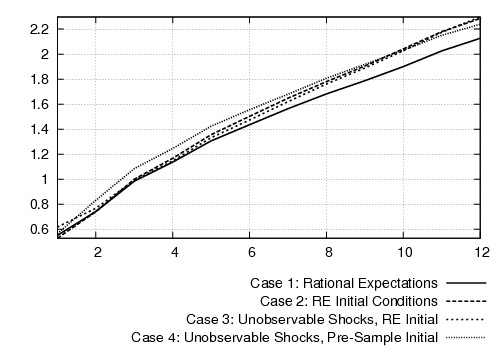
\includegraphics[scale=0.55]{output_fore.png} \\ 
Inflation \\ 
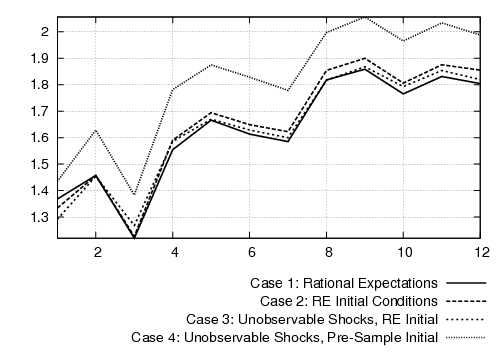
\includegraphics[scale=0.55]{inflation_fore.png} \\ 
Federal Funds Rate \\ 
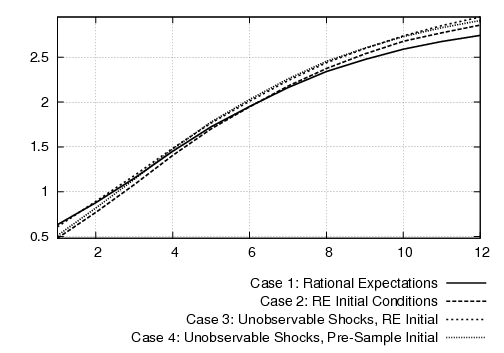
\includegraphics[scale=0.55]{fedfunds_fore.png} \\ 
\end{tabular}
\end{center}
\end{figure}

\begin{figure}
\caption{Smoothed Estimates of Structural Shocks}\label{fg:shocks}
\vspace*{1pc}\hspace*{-0.2in}
\begin{tabular}{ccc}
\multicolumn{3}{c}{Case 1: Rational Expectations} \\ 
Natural Rate & Cost-Push & Monetary Policy \\
\includegraphics[scale=0.3]{results_re/natrateshock.png} & 
\includegraphics[scale=0.3]{results_re/costpushshock.png} & 
\includegraphics[scale=0.3]{results_re/mpshock.png} \\ \\ 
 
\multicolumn{3}{c}{Case 2: Learning with RE Initial Conditions} \\ 
Natural Rate (0.9752) & Cost-Push (0.9434) & Monetary Policy (0.9629) \\
\includegraphics[scale=0.3]{results_reallinit/natrateshock.png} & 
\includegraphics[scale=0.3]{results_reallinit/costpushshock.png} & 
\includegraphics[scale=0.3]{results_reallinit/mpshock.png} \\ \\ 
 
\multicolumn{3}{c}{Case 3: Learning with Unobservable Shocks and RE Initial Conditions} \\ 
Natural Rate (0.8366) & Cost-Push (0.9343) & Monetary Policy (0.8062) \\
\includegraphics[scale=0.3]{results_reinit/natrateshock.png} & 
\includegraphics[scale=0.3]{results_reinit/costpushshock.png} & 
\includegraphics[scale=0.3]{results_reinit/mpshock.png} \\ \\ 
 
\multicolumn{3}{c}{Case 4: Learning with Unobservable Shocks and Pre-Sample Initial Conditions} \\ 
Natural Rate (0.6217) & Cost-Push (0.9071) & Monetary Policy (0.8383) \\
\includegraphics[scale=0.3]{results_wlsinit/natrateshock.png} & 
\includegraphics[scale=0.3]{results_wlsinit/costpushshock.png} & 
\includegraphics[scale=0.3]{results_wlsinit/mpshock.png} \\ \\ 
 
\end{tabular}
\end{figure}

\begin{figure}
\caption{Natural Rate Shock Impulse Responses}\label{fg:irf_nat}
\vspace*{1pc}
\begin{tabular}{ccc}
\multicolumn{3}{c}{Case 1: Rational Expectations}\\
Output Gap & Inflation & Interest Rate \\ 
\includegraphics[scale=0.28]{results_re/Output_natshock_irf.png} & 
\includegraphics[scale=0.28]{results_re/Inflation_natshock_irf.png} & 
\includegraphics[scale=0.28]{results_re/Interest_Rate_natshock_irf.png} \\ \\ 
\multicolumn{3}{c}{Case 2: Learning with RE Initial Conditions}\\
Output Gap & Inflation & Interest Rate \\ 
\includegraphics[scale=0.28]{results_reallinit/Output_natshock_irf.png} & 
\includegraphics[scale=0.28]{results_reallinit/Inflation_natshock_irf.png} & 
\includegraphics[scale=0.28]{results_reallinit/Interest_Rate_natshock_irf.png} \\ \\ 
\multicolumn{3}{c}{Case 3: Learning with Unobservable Shocks and RE Initial Conditions}\\
Output Gap & Inflation & Interest Rate \\ 
\includegraphics[scale=0.28]{results_reinit/Output_natshock_irf.png} & 
\includegraphics[scale=0.28]{results_reinit/Inflation_natshock_irf.png} & 
\includegraphics[scale=0.28]{results_reinit/Interest_Rate_natshock_irf.png} \\ \\ 
\multicolumn{3}{c}{Case 4: Learning with Unobservable Shocks and Pre-Sample Initial Conditions}\\
Output Gap & Inflation & Interest Rate \\ 
\includegraphics[scale=0.28]{results_wlsinit/Output_natshock_irf.png} & 
\includegraphics[scale=0.28]{results_wlsinit/Inflation_natshock_irf.png} & 
\includegraphics[scale=0.28]{results_wlsinit/Interest_Rate_natshock_irf.png} \\ 
\end{tabular}
\end{figure}

\begin{figure}
\caption{Cost-Push Shock Impulse Responses}\label{fg:irf_cost}
\vspace*{1pc}
\begin{tabular}{ccc}
\multicolumn{3}{c}{Case 1: Rational Expectations}\\
Output Gap & Inflation & Interest Rate \\ 
\includegraphics[scale=0.28]{results_re/Output_costshock_irf.png} & 
\includegraphics[scale=0.28]{results_re/Inflation_costshock_irf.png} & 
\includegraphics[scale=0.28]{results_re/Interest_Rate_costshock_irf.png} \\ \\ 
\multicolumn{3}{c}{Case 2: Learning with RE Initial Conditions}\\
Output Gap & Inflation & Interest Rate \\ 
\includegraphics[scale=0.28]{results_reallinit/Output_costshock_irf.png} & 
\includegraphics[scale=0.28]{results_reallinit/Inflation_costshock_irf.png} & 
\includegraphics[scale=0.28]{results_reallinit/Interest_Rate_costshock_irf.png} \\ \\ 
\multicolumn{3}{c}{Case 3: Learning with Unobservable Shocks and RE Initial Conditions}\\
Output Gap & Inflation & Interest Rate \\ 
\includegraphics[scale=0.28]{results_reinit/Output_costshock_irf.png} & 
\includegraphics[scale=0.28]{results_reinit/Inflation_costshock_irf.png} & 
\includegraphics[scale=0.28]{results_reinit/Interest_Rate_costshock_irf.png} \\ \\ 
\multicolumn{3}{c}{Case 4: Learning with Unobservable Shocks and Pre-Sample Initial Conditions}\\
Output Gap & Inflation & Interest Rate \\ 
\includegraphics[scale=0.28]{results_wlsinit/Output_costshock_irf.png} & 
\includegraphics[scale=0.28]{results_wlsinit/Inflation_costshock_irf.png} & 
\includegraphics[scale=0.28]{results_wlsinit/Interest_Rate_costshock_irf.png} \\ 
\end{tabular}
\end{figure}

\begin{figure}
\caption{Monetary Policy Shock Impulse Responses}\label{fg:irf_mp}
\vspace*{1pc}
\begin{tabular}{ccc}
\multicolumn{3}{c}{Case 1: Rational Expectations}\\
Output Gap & Inflation & Interest Rate \\ 
\includegraphics[scale=0.28]{results_re/Output_mpshock_irf.png} & 
\includegraphics[scale=0.28]{results_re/Inflation_mpshock_irf.png} & 
\includegraphics[scale=0.28]{results_re/Interest_Rate_mpshock_irf.png} \\ \\ 
\multicolumn{3}{c}{Case 2: Learning with RE Initial Conditions}\\
Output Gap & Inflation & Interest Rate \\ 
\includegraphics[scale=0.28]{results_reallinit/Output_mpshock_irf.png} & 
\includegraphics[scale=0.28]{results_reallinit/Inflation_mpshock_irf.png} & 
\includegraphics[scale=0.28]{results_reallinit/Interest_Rate_mpshock_irf.png} \\ \\ 
\multicolumn{3}{c}{Case 3: Learning with Unobservable Shocks and RE Initial Conditions}\\
Output Gap & Inflation & Interest Rate \\ 
\includegraphics[scale=0.28]{results_reinit/Output_mpshock_irf.png} & 
\includegraphics[scale=0.28]{results_reinit/Inflation_mpshock_irf.png} & 
\includegraphics[scale=0.28]{results_reinit/Interest_Rate_mpshock_irf.png} \\ \\ 
\multicolumn{3}{c}{Case 4: Learning with Unobservable Shocks and Pre-Sample Initial Conditions}\\
Output Gap & Inflation & Interest Rate \\ 
\includegraphics[scale=0.28]{results_wlsinit/Output_mpshock_irf.png} & 
\includegraphics[scale=0.28]{results_wlsinit/Inflation_mpshock_irf.png} & 
\includegraphics[scale=0.28]{results_wlsinit/Interest_Rate_mpshock_irf.png} \\ 
\end{tabular}
\end{figure}

\begin{figure}
\caption{Natural Rate Shock Impulse Responses}\label{fg:irf_nat}
\vspace*{1pc}
\begin{tabular}{cc}
\multicolumn{2}{c}{Case 2: Learning with RE Initial Conditions}\\ \\
Output Gap & Inflation \\ 
\includegraphics[scale=0.25]{results_reallinit/Output_natshock_irf3d.png} & 
\includegraphics[scale=0.25]{results_reallinit/Inflation_natshock_irf3d.png} \\ \\ 
\multicolumn{2}{c}{Case 3: Learning with Unobservable Shocks and RE Initial Conditions}\\ \\
Output Gap & Inflation \\ 
\includegraphics[scale=0.25]{results_reinit/Output_natshock_irf3d.png} & 
\includegraphics[scale=0.25]{results_reinit/Inflation_natshock_irf3d.png} \\ \\ 
\multicolumn{2}{c}{Case 4: Learning with Unobservable Shocks and Pre-Sample Initial Conditions}\\ \\
Output Gap & Inflation \\ 
\includegraphics[scale=0.25]{results_wlsinit/Output_natshock_irf3d.png} & 
\includegraphics[scale=0.25]{results_wlsinit/Inflation_natshock_irf3d.png} \\ 
\end{tabular}
\end{figure}

\begin{figure}
\caption{Cost-Push Shock Impulse Responses}\label{fg:irf_cost}
\vspace*{1pc}
\begin{tabular}{cc}
\multicolumn{2}{c}{Case 2: Learning with RE Initial Conditions}\\ \\
Output Gap & Inflation \\ 
\includegraphics[scale=0.25]{results_reallinit/Output_costshock_irf3d.png} & 
\includegraphics[scale=0.25]{results_reallinit/Inflation_costshock_irf3d.png} \\ \\ 
\multicolumn{2}{c}{Case 3: Learning with Unobservable Shocks and RE Initial Conditions}\\ \\
Output Gap & Inflation \\ 
\includegraphics[scale=0.25]{results_reinit/Output_costshock_irf3d.png} & 
\includegraphics[scale=0.25]{results_reinit/Inflation_costshock_irf3d.png} \\ \\ 
\multicolumn{2}{c}{Case 4: Learning with Unobservable Shocks and Pre-Sample Initial Conditions}\\ \\
Output Gap & Inflation \\ 
\includegraphics[scale=0.25]{results_wlsinit/Output_costshock_irf3d.png} & 
\includegraphics[scale=0.25]{results_wlsinit/Inflation_costshock_irf3d.png} \\ 
\end{tabular}
\end{figure}

\begin{figure}
\caption{Monetary Policy Shock Impulse Responses}\label{fg:irf_mp}
\vspace*{1pc}
\begin{tabular}{cc}
\multicolumn{2}{c}{Case 2: Learning with RE Initial Conditions}\\ \\
Output Gap & Inflation \\ 
\includegraphics[scale=0.25]{results_reallinit/Output_mpshock_irf3d.png} & 
\includegraphics[scale=0.25]{results_reallinit/Inflation_mpshock_irf3d.png} \\ \\ 
\multicolumn{2}{c}{Case 3: Learning with Unobservable Shocks and RE Initial Conditions}\\ \\
Output Gap & Inflation \\ 
\includegraphics[scale=0.25]{results_reinit/Output_mpshock_irf3d.png} & 
\includegraphics[scale=0.25]{results_reinit/Inflation_mpshock_irf3d.png} \\ \\ 
\multicolumn{2}{c}{Case 4: Learning with Unobservable Shocks and Pre-Sample Initial Conditions}\\ \\
Output Gap & Inflation \\ 
\includegraphics[scale=0.25]{results_wlsinit/Output_mpshock_irf3d.png} & 
\includegraphics[scale=0.25]{results_wlsinit/Inflation_mpshock_irf3d.png} \\ 
\end{tabular}
\end{figure}

%\begin{figure}
\caption{Agents' Expectations}\label{fg:exp}\vspace*{1pc}\hspace*{-0.35in}
\begin{tabular}{cc}
\multicolumn{2}{c}{Case 2: Expectations with RE Initial Conditions} \\ 
Output Gap & Inflation \\
\includegraphics[scale=0.48]{results_reallinit/output_exp.png} & 
\includegraphics[scale=0.48]{results_reallinit/inflation_exp.png} \\ \\ 
 
\multicolumn{2}{c}{Case 3: Expectations with with Unobservable Shocks and RE Initial Conditions} \\ 
Output Gap & Inflation \\
\includegraphics[scale=0.48]{results_reinit/output_exp.png} & 
\includegraphics[scale=0.48]{results_reinit/inflation_exp.png} \\ \\ 
 
\multicolumn{2}{c}{Case 4: Expectations with Unobservable Shocks and Pre-Sample Initial Conditions} \\ 
Output Gap & Inflation \\
\includegraphics[scale=0.48]{results_wlsinit/output_exp.png} & 
\includegraphics[scale=0.48]{results_wlsinit/inflation_exp.png} \\ \\ 
 
\end{tabular}
\end{figure}



\end{document}



